\section{Theory}
%\label{sec:problem_description}
In Experiment A, the basic equations are Bernoulli's \eqref{Bernoulli} .
%and the continuity equation.

\begin{equation}
\label{Bernoulli}
\left[ \frac{p}{\gamma}+\frac{v^2}{2g}+z \right]_1 = 
\left[ \frac{p}{\gamma}+\frac{v^2}{2g}+z \right]_2 
\end{equation}

As shown in the figure below, where 1 and 2 represent the surface of 
the reservoir and the water discharge point.

\begin{figure}[htb] % Here, top, bottom priority list
    \centering
    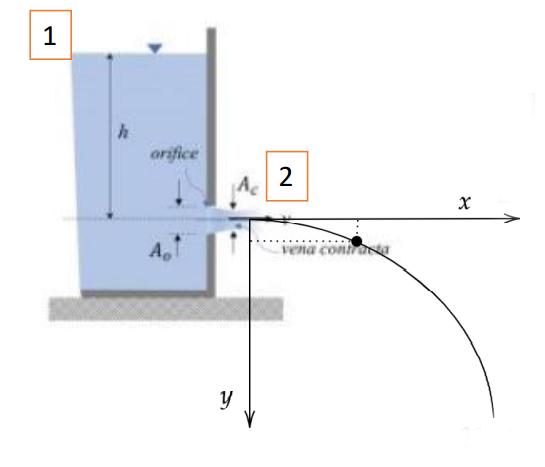
\includegraphics[scale=0.45]{Theory/figures/figure1.png}
    \caption{Experimental Demonstration}
    \label{fig:demo}
\end{figure}

In Bernoulli's equation, because the position 1 is in contact with the air and the water surface is static, 
so the pressure force p = 0, and the water surface flow velocity v = 0. 
Similarly, the pressure at position 2 is p = 0. 
With the datum at 2, we only need to measure the head difference between position 1 and 2, 
and measure the jet velocity of 2, after that put into other constants, 
Bernoulli's equation could be proved.










In Experiment B, it provides a method to measure the velocity of the water jet at position 2. 
The water flow rate is calculated by measuring the volume of water flowing out in a certain time 
by the formula \eqref{Flow}.

\begin{equation}
\label{Flow}
Q=\frac{V}{T}
\end{equation}

Further more, the continuity equation \eqref{velocity} enables to calculate the water jet velocity.

\begin{equation}
\label{velocity}
Q=Av
\end{equation}

From this, we can calculate the real water jet velocity.

Notice:  the water jet velocity measured by experiment A exists a 
certain error.
The flow rate measured by experiment B is a relatively smaller error.
(see in section: Analysis %\autoref{sec:analysis}
)